%LaTex cheat sheet template
\documentclass[10pt,a4paper,landscape]{article}

\usepackage[utf8]{inputenc}
\usepackage{amsmath}
% \usepackage{amsfonts}
% \usepackage{amssymb}
% \usepackage{xfrac}
\usepackage{multicol}
\usepackage{geometry}
% \usepackage{lipsum}
\usepackage{titlesec}
\usepackage[nodisplayskipstretch]{setspace}
% \usepackage{enumitem}
\usepackage{graphicx}
\usepackage{wrapfig}
\usepackage{minted}
% \usepackage{float}
\usepackage{enumitem}
\usepackage{booktabs}
\usepackage{tabularx}

%rainbow_dash
%emacs
%perldoc
\usemintedstyle{perldoc}
\setminted{
    breaklines=true,
    fontsize=\normalsize
}

\geometry{a4paper, left=0mm, top=0mm, right=0mm, bottom=1mm}

\titlespacing{\section}{0pt}{0pt}{0pt}
\titlespacing{\subsection}{0pt}{0pt}{0pt}
\titlespacing{\subsubsection}{0pt}{0pt}{0pt}

\setlength{\abovedisplayskip}{0pt}
\setlength{\belowdisplayskip}{0pt}
\setlength{\parindent}{0pt}

\setlist[itemize]{itemsep=0pt, topsep=0pt, partopsep=0pt}

%\renewcommand{\normalsize}{\footnotesize} % set global font size to footnotesize

\begin{document}
\begin{multicols*}{3}
    \section*{AdvEmbSoft}
    \subsection*{C++}
Initializes a vector \texttt{v} with four integers and uses a range-based
for loop to print each element. The \texttt{auto} keyword automatically deduces
the element type (\texttt{int} in this case).
\begin{minted}{c++}
std::vector<int> v = {7, 5, 16, 8};
for (auto n : v) {
    std::cout << n << " ";
}
\end{minted}

Objects can be allocated on the stack or heap.\texttt{s1} and \texttt{s2} are stack-allocated
strings, while \texttt{s3} is a heap-allocated string. \texttt{s4} is a deep copy of \texttt{s2},
and \texttt{s5} is a shallow copy of \texttt{s3}. Changes to \texttt{s5} affect \texttt{s3}, as
shown by changing the first character to '@'. Heap memory is deallocated with \texttt{delete}.
\begin{minted}{c++}
std::string s1; //empty string
std::string s2("Hello"); //initialized string
std::string* s3 = new std::string("World"); //heap string
std::string s4 = s2; //deep copy
std::string* s5 = s3; //shallow copy
s5->at(0) = '@'; //s3 is also modified
delete s3; s3 = nullptr; //heap deallocation
delete s5; s5 = nullptr; 
\end{minted}

Declares two global variables. \texttt{globalVariable} can be accessed from any
part of the program, while \texttt{restrictedGlobalVariable} is \texttt{static},
limiting its scope to this file only.
\begin{minted}{c++}
int globalVariable = 9;
static int restrictedGlobalVariable = 10;
\end{minted}

Declares global constants and class constants. \texttt{kGlobalConstantExpr} is a
compile-time constant, while \texttt{kGlobalConstant} is a runtime constant. Inside
\texttt{ClassWithConstant}, \texttt{kConstantExpr} is a compile-time constant, and
\texttt{kConstant} is a runtime constant initialized with \texttt{kGlobalConstant * 2}.
\begin{minted}{c++}
static constexpr uint32_t kGlobalConstantExpr = 1;
static const uint32_t kGlobalConstant = rand();
class ClassWithConstant {
public:
    static constexpr uint32_t kConstantExpr = 2;
    static const uint32_t kConstant;
};
const uint32_t ClassWithConstant::kConstant = kGlobalConstant * 2;
\end{minted}

Demonstrates the use of fixed and dynamic arrays. \texttt{myArray1} is a
fixed-size array on the stack, while \texttt{myArray2} is a dynamically allocated array on
the heap. \texttt{myArray} is a dynamic array whose size is determined at runtime. The
\texttt{sizeof} operator is used to calculate the size of \texttt{myArray}.
\begin{minted}{c++}
static constexpr int arraySize = 30;
int myArray1[arraySize] = {0}; //fixed array on stack
int* myArray2 = new int[arraySize];  //dynamic array on heap
delete[] myArray2; //realease heap memory
myArray2 = nullptr; //reset pointer
int varSize = 5;
int myArray[varSize] = {0};
myArray[0] = 1;
myArray[1] = myArray[0];
int size = sizeof(myArray) / sizeof(int);
\end{minted}

Demonstrates the use of a \texttt{std::vector}, a dynamic array. It initializes
\texttt{v} with four integers, adds two more at the end, removes the last one, and accesses the
first and last elements. It also gets the size of the vector.
\begin{minted}{c++}
std::vector<int> v = {7, 5, 16, 8};
v.push_back(25); //add element to end
v.push_back(13); //add another element to end
v.pop_back(); //remove last element
std::cout << "First element is : " << v.front() << std::endl;
std::cout << "Last element is : " << v.back() << std::endl;
int size = v.size();
\end{minted}

Two ways to create a 2D array. The first part uses raw pointers to create
a jagged array, where each row has a different length. The second part uses \texttt{std::vector},
a dynamic array from the C++ Standard Library, to achieve the same result in a safer and simpler way.
\begin{minted}{c++}
char** array = new char*[base]; //jagged array
for (int i = 0; i < base; i++) {
    array[i] = new char[base - i + 1];
    for (int j = 0; j < base - i; j++){
        array[i][j] = '*';
    }
    array[i][base - i] = '\0';
}

std::vector<std::vector<char>> array(base); //2D vector
for (int i = 0; i < base; i++){
    array[i] = std::vector<char>(base - i, '*');
}
\end{minted}

Defines a \texttt{Point} class with two constructors, methods to move the point and
access its coordinates, and an operator overload for addition. The `+` operator is overloaded to
add the coordinates of two points.
\begin{minted}{c++}
class Point {
    public:
        Point() : _x(0), _y(0) { } // constructors
        Point(float x, float y) : _x(x), _y(y) { }
        ~Point() { // destructor
            std::cout << "Point destructor called" << std::endl;
        }
        void move(float dx, float dy) { // public methods
            _x += dx;
            _y += dy;
        }
        float x() const { return _x; }
        float y() const { return _y; }
        Point operator+(const Point& other) const {
            return Point(_x + other._x, _y + other._y);
        }
    private:
        float _x; // private data fields
        float _y;
};
\end{minted}

Demonstrates the concept of polymorphism. It defines a \texttt{Base} class and a
\texttt{Derived} class that inherits from \texttt{Base}. Both classes have a method \texttt{f()},
but in \texttt{Derived}, \texttt{f()} is overridden. When \texttt{f()} is called on a \texttt{Base}
reference or pointer that actually points to a \texttt{Derived} object, the \texttt{Derived}
version of \texttt{f()} is called due to the \texttt{virtual} keyword.
\begin{minted}{c++}
class Base {
public:
    virtual void f() {
        std::cout << "f() in Base class called" << std::endl;
    }
};
class Derived : public Base {
public:
    void f() override {
        std::cout << "f() in Derived class called" << std::endl;
    }
};
int main() {
    Base b; // Create a base instance
    Derived d; // Create a derived instance
    b.f(); // Prints base
    d.f(); // Prints derived
    Base& br = b; // The type of br is Base&
    Base& dr = d; // The type of dr is Base& as well
    br.f(); // Prints base
    dr.f(); // Prints derived (because Base::f() is declared as virtual)
    Base* bp = &b; // The type of bp is Base*
    Base* dp = &d; // The type of dp is Base* as well
    bp->f(); // Prints base
    dp->f(); // Prints derived (because Base::f() is declared as virtual)
    br.Base::f(); // prints base
    dr.Base::f(); // prints base
    return 0;
}
\end{minted}

Defines a \texttt{Buffer} class that allocates a block of memory when it is
constructed and releases that memory when it is destroyed. This is a common pattern for classes
that manage resources, which is often referred to as Resource Acquisition Is Initialization (RAII).
\begin{minted}{c++}
class Buffer {
public:
    Buffer(size_t size) : _size(size), _data(new char[size]) { }
    ~Buffer() { // destructor
        delete[] _data; // release the allocated memory
    }
private:
    size_t _size;
    char* _data;
};
\end{minted}

Demonstrates two ways of managing dynamic memory. The first part uses raw pointers to
allocate and deallocate memory manually, which can lead to memory leaks if not handled properly.
The second part uses \texttt{std::unique\_ptr}, a smart pointer that automatically deallocates the
memory when it's no longer needed, preventing memory leaks.
\begin{minted}{c++}
void function()
{
    char* pArray = new char[100]; // solution with raw pointer
    bool condition = false;
    if (condition) {
        // at this point, a memory leak arises since pArray is not released
        return;
    }
    delete [] pArray;
    pArray = nullptr;
    // solution with unique_ptr
    std::unique_ptr<char[]> array_ptr(new char[99]);
    if (condition) {
        // no memory leak since the destructor of array_ptr is called
        return;
    }
}
\end{minted}

Class templates allow for creating classes that can work with different data types and sizes.
The \texttt{Arithmetic<T>} class performs basic arithmetic operations on any type \texttt{T}. The
\texttt{Queue<T, queue\_sz>} class represents a queue of any type \texttt{T} with a size
\texttt{queue\_sz} known at compile time.
\begin{minted}{c++}
template <class T> class Arithmetic {
public:
    Arithmetic(T a, T b) : _a(a), _b(b) {}
    T add() { return _a + _b; }
    T sub() { return _a - _b; }
private:
    T _a, _b;
};
template <typename T, uint32_t queue_sz> class Queue {
public:
    uint32_t getSize() const { return queue_sz;}
private:
    T array[queue_sz];
};
int main() {
    Arithmetic<float> a2(1.5, 2.1);
    Queue<int, 10> intQueue;
    return 0;
}
\end{minted}
    \subsection*{Scheduling}
\underline{Timing constraints:}\\
Deadline: D\\
Arrival time: A\\
Release time: R\\
Finish time: F\\
Computation time: C\\
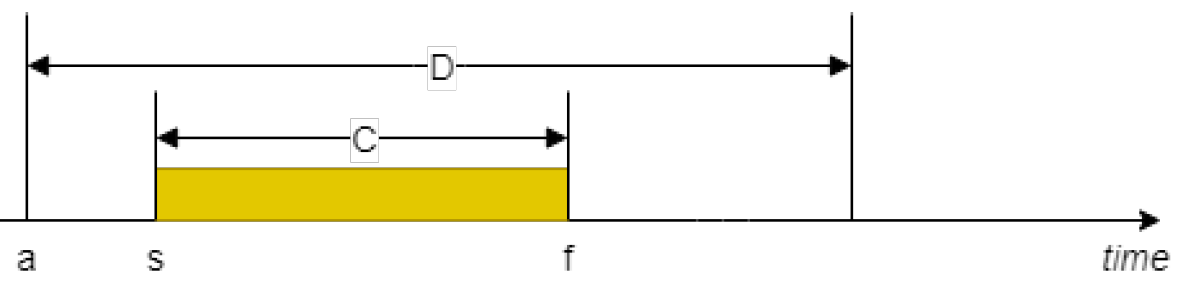
\includegraphics[width=\columnwidth]{images/timing_constraints.png}
\textit{Task response time} $=f-a$ ou $f-r$\\
\textit{Maximum lateness} $=\max_i(f_i-d_i)$\\
\textit{Maximum number of late tasks}
$=\sum_{i=1}^{n} \text{miss}(f_i)=
    \begin{cases}
        0 & \text{if } f_i \leq d_i \\
        1 & \text{otherwise}
    \end{cases}$\\
\textit{Schedulability:} $U=\sum_{i=1}^{n} \frac{C_i}{T_i} \leq 1$\\
Can be increased by increasing task computation times or by decreasing their periods.\\
\textbf{Time cyclic scheduling:}\\
Divide the temporal axis into slots of equal length (length = Minor Cycle).
The optimal length of the Minor Cycle is the GCD (=plus grand diviseur commun) of the periods.
The optimal length of the Major Cycle is the LCM (=plus petit multiple commun) of the periods.
If tasks cannot be split into sub-tasks, then a set of tasks is schedulable if
the sum of execution times within each time slot is less or equal to the Minor
Cycle.\\
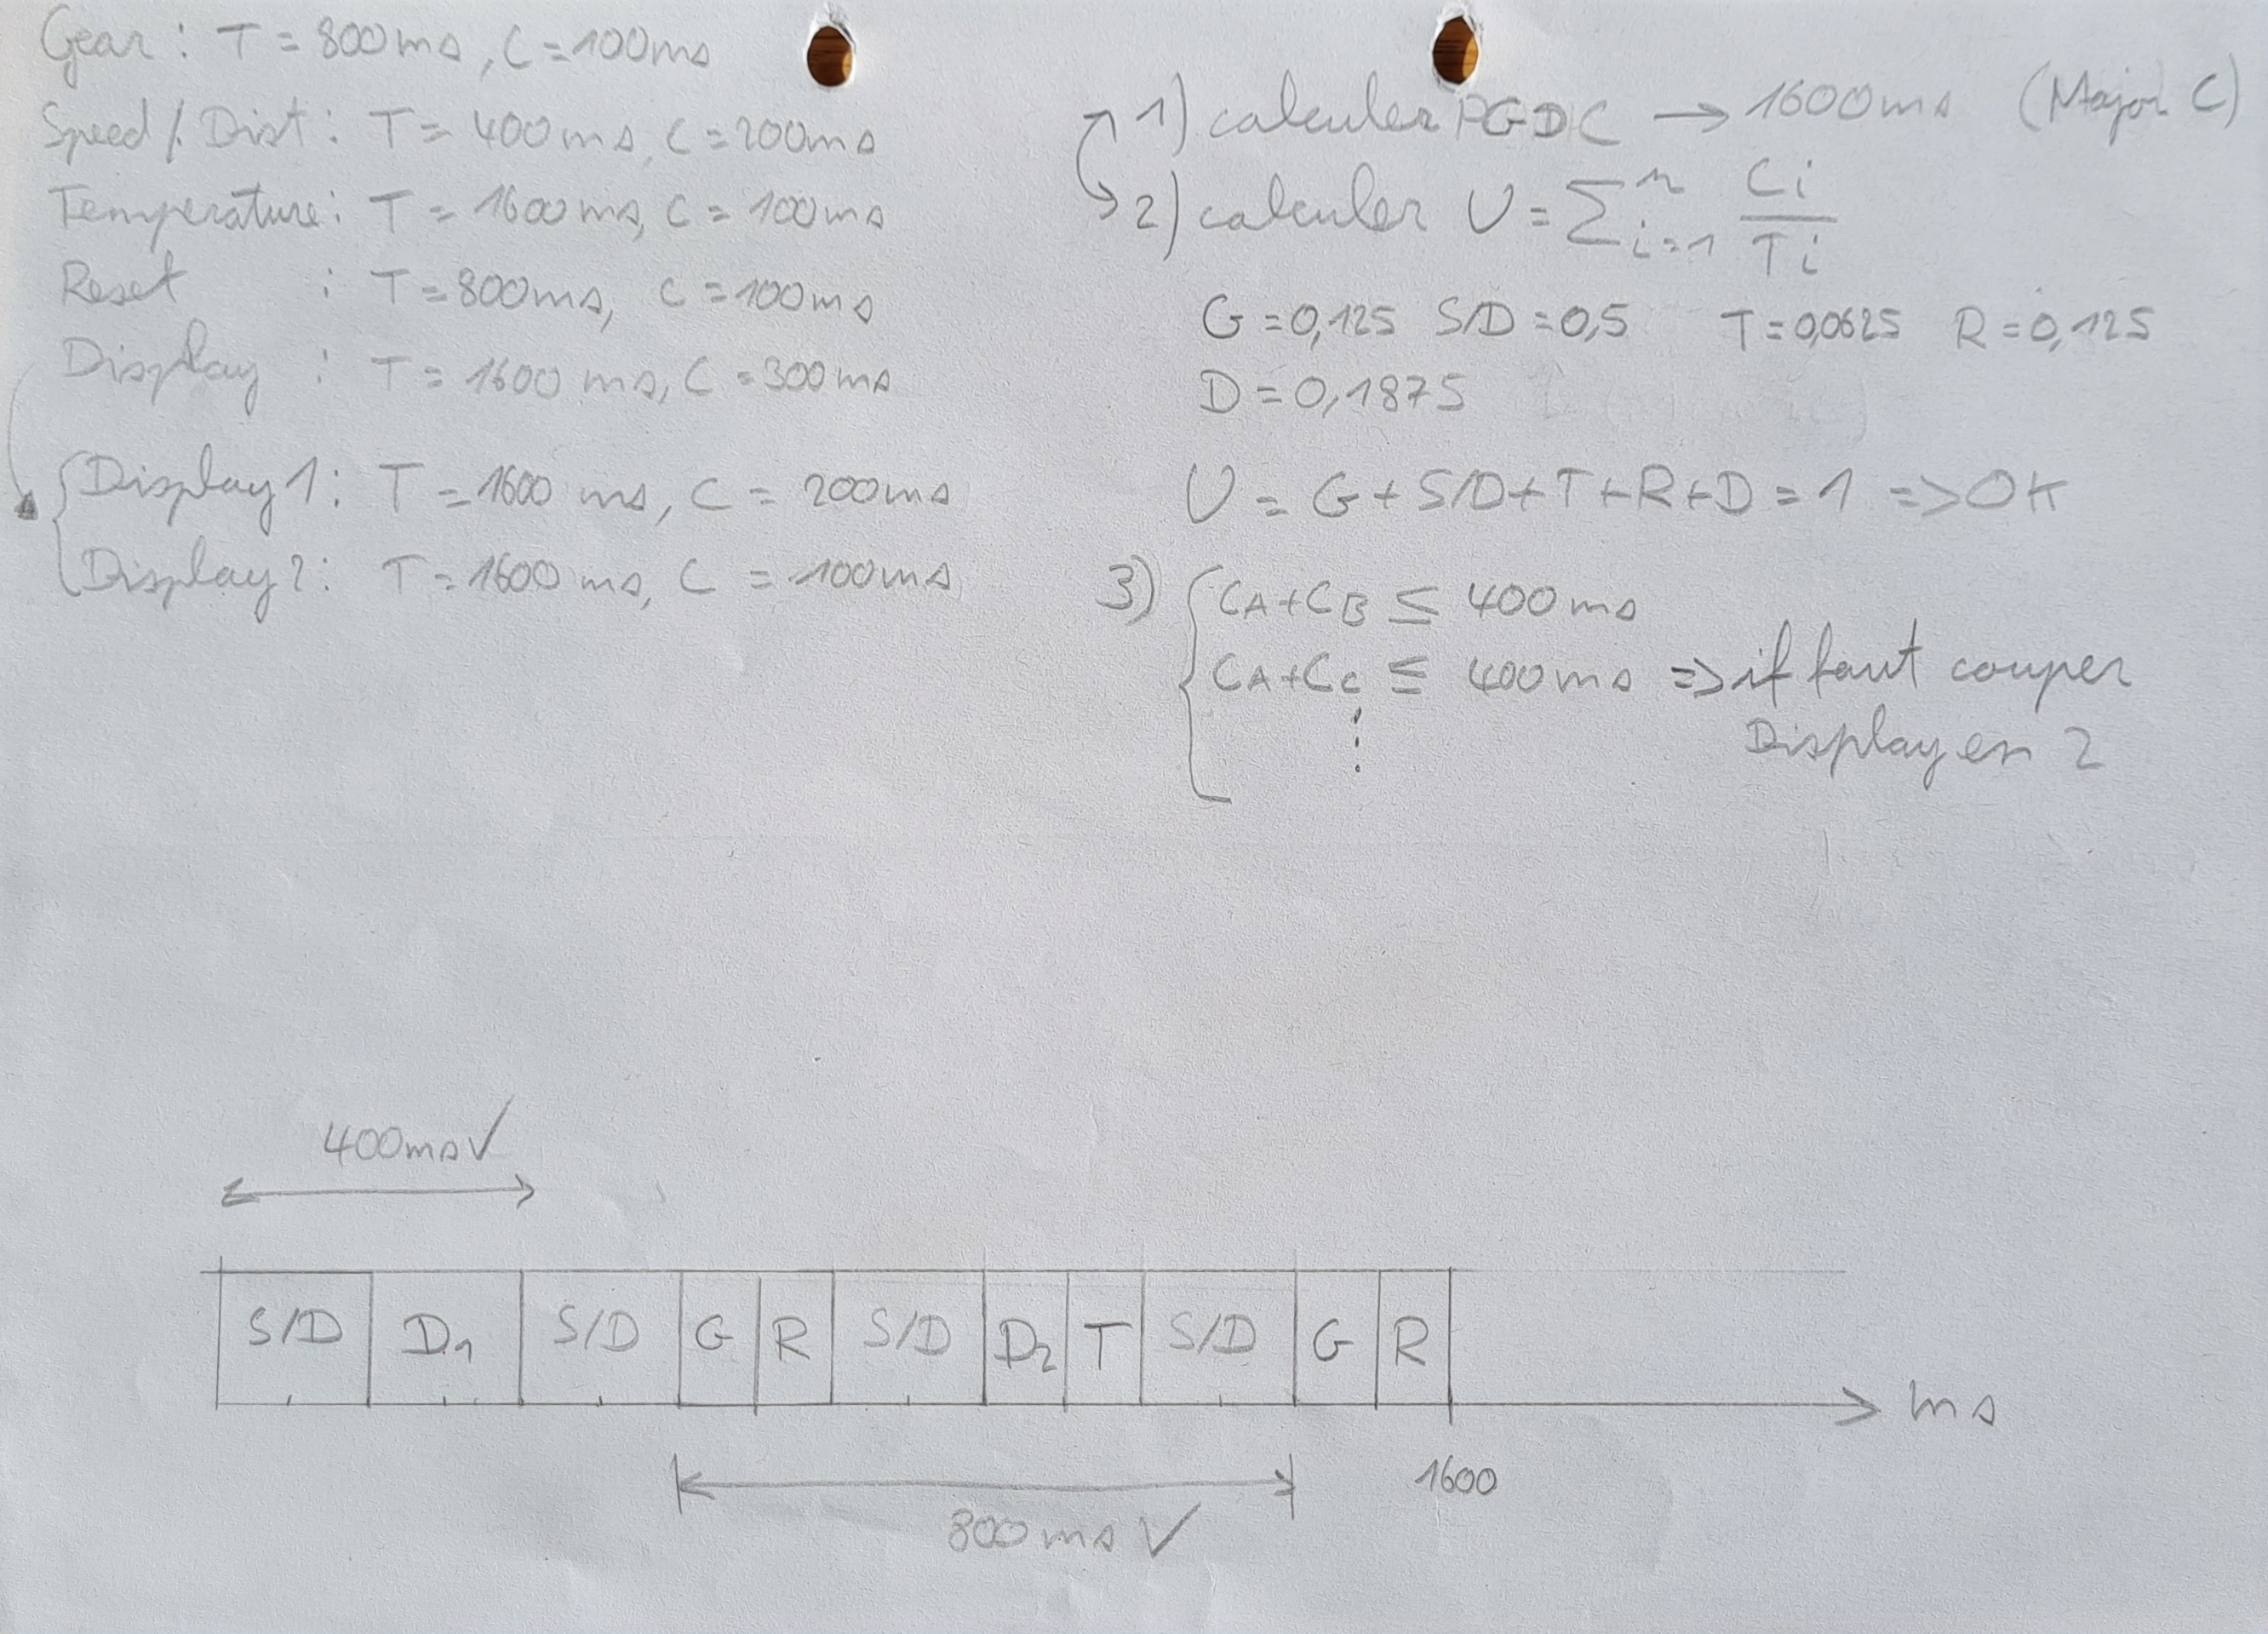
\includegraphics[width=\columnwidth]{images/time_cyclic_scheduling.jpg}
Advantages:
\begin{itemize}
    \item Easy to implement
    \item Predictable
    \item No need for a scheduler
\end{itemize}
Disadvantages:
\begin{itemize}
    \item Always run the same schedule
    \item The polling rate is limited by 1/maximum delay.
    \item The program must continually check the status of every device
    \item This approach scales badly
\end{itemize}
\textbf{Event-driven systems:}\\
Handling events is done using interrupts. Interrupts can be prioritized.
Interrupts can be masked: switched off if not needed or likely to get in the way of more
important activity. Interrupts can be nested. The location of the ISR in memory can be selected.\\
%put two images side by side 
\begin{minipage}{.49\columnwidth}
    \centering
    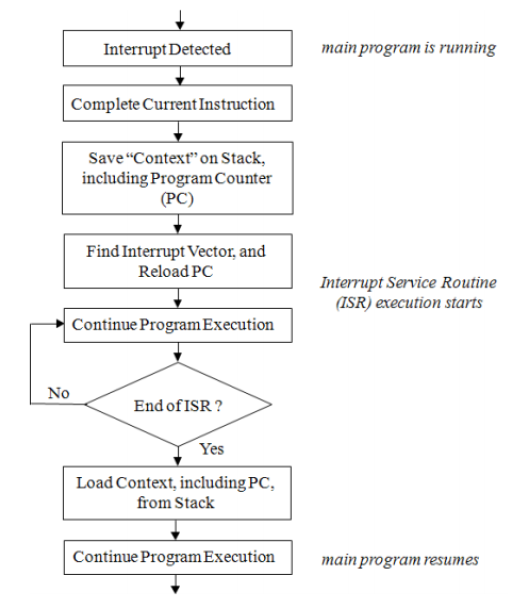
\includegraphics[width=\linewidth]{images/interrupt1.png}
\end{minipage}
\begin{minipage}{.49\columnwidth}
    \centering
    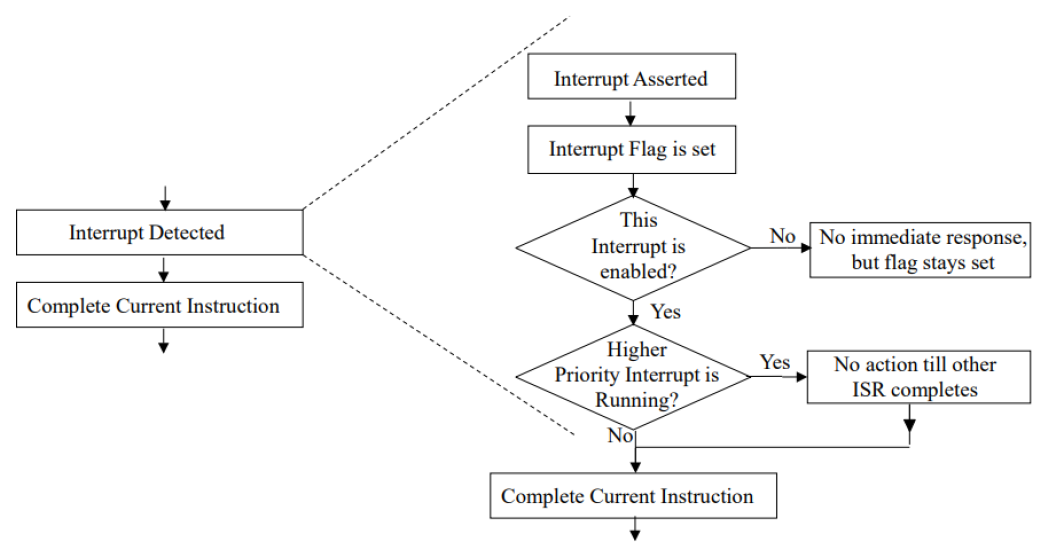
\includegraphics[width=\linewidth,height=\linewidth,keepaspectratio=false]{images/interrupt2.png} % set height to \linewidth
\end{minipage}\\
\textbf{Dynamic scheduling:}\\
Allows task scheduling to be computed dynamically online based on importance or any other
criteria such as task deadline, duration, or creation time.\\
\underline{Task preemption:}\\
Exception handling/interrupt may need to preempt existing tasks.
Suspend a running task and insert it in the ready queue. Schedule tasks based on their
priority/importance. Improve efficiency.\\
Advantages:
\begin{itemize}
    \item Better response time
    \item Can do more processing
    \item Can lower processor speed, saving money and power
\end{itemize}
Disadvantages:
\begin{itemize}
    \item More complicated programming
    \item More memory.
    \item Introduces vulnerability
\end{itemize}
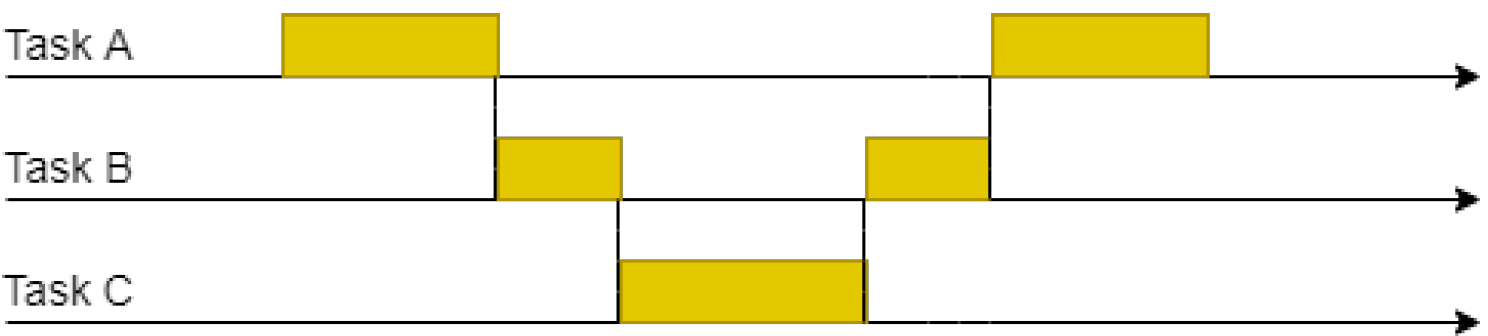
\includegraphics[width=\columnwidth]{images/preemption.png}
\underline{Rate Monotonic Scheduling:}\\
Tasks with higher request rates/shorter periods have higher priorities.
Fixed periods means fixed priorities. Is optimal among fixed-priority algorithms.
\textit{Schedulability:} $U=\sum_{i=1}^{n} \frac{C_i}{T_i} \leq n(2^{\frac{1}{n}}-1)$\\
\underline{Earliest Deadline First:}\\
Tasks with earlier deadlines have higher priorities.
Priorities are dynamic since absolute deadlines of periodic tasks vary over time.
\textit{Schedulability:} $U=\sum_{i=1}^{n} \frac{C_i}{T_i} \leq 1$\\

    \subsection*{Tasks and concurrency}
A \underline{task} is a set of program instructions, a \underline{process} is an instance of a computer program that
is being executed, and a \underline{thread} is a basic unit of CPU utilization that can exist within a
process. Meaning a thread consists of a program counter, a stack, and a set of registers.\\
Each thread has its own stack, but all threads in a process share the same heap. The stack is
used for storing temporary data that is created and destroyed during the execution of a
function, while the heap is used for storing data that needs to persist beyond the lifetime of
a function.
% \begin{wrapfigure}{r}{0.5\columnwidth}
%     \centering
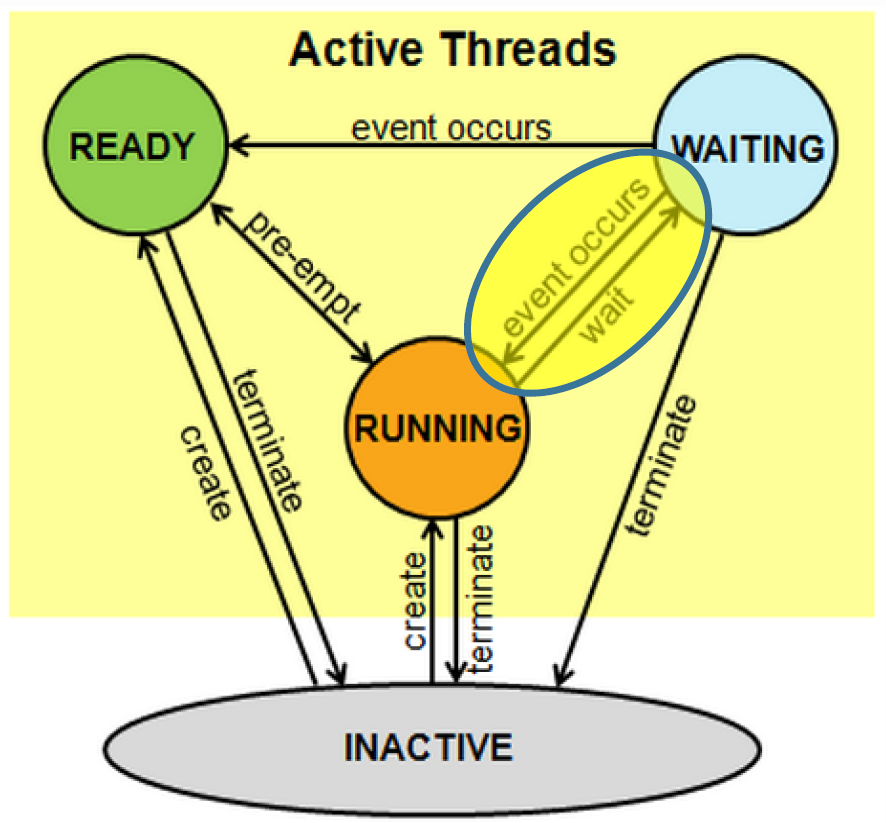
\includegraphics[width=\columnwidth]{images/thread_states.png}
% \end{wrapfigure}
In a multitasking system, the different tasks may compete for shared resources or may wait for
different events to happen. In some cases, a given task may thus enter a Waiting or Blocked state.\\
\underline{Mutex:} only one thread can access a shared resource at a time.
\begin{minted}{c++}
Mutex mtx;
mtx.lock();
//critical section
mtx.unlock();
\end{minted}
\underline{Semaphore:}\\
A semaphore is a synchronization object that controls access to a shared resource by multiple
threads. Unlike a mutex, a semaphore can control access to several shared resources.
\begin{minted}{c++}
Semaphore sem_in {2};
Semaphore sem_out {0};
sem_in.acquire(); //decrement
//critical section
sem_out.release(); //increment
\end{minted}
\underline{Deadlock:}\\
A deadlock is a situation where two or more competing tasks are waiting for each other to
finish, and thus neither ever does.\\
\underline{Queue/Mail:}\\
A queue is a FIFO data structure that can be used to pass messages between tasks.\\
    \subsection*{Priority inversion}
Priority inversion occurs when a higher-priority task is waiting for a resource held by a
lower-priority task. The main sources of priority inversion are non preemptable sections,
sharing resources. synchronization and mutual exclusion. The solution is to use Resource
Access Protocols\\
\underline{Non-Preemptive Protocol (NPP)}\\
A task is assigned the highest priority if it succeeds in locking a critical section.
The task is assigned its own priority when it releases the critical section.\\
Advantages:
\begin{itemize}
    \item Bounds(= limite) Priority Inversion and for a given task the bound is the maximal length
          of any single critical section belonging to lower priority tasks.
    \item It is deadlock free and limits the number of blocking of any task to one.
\end{itemize}
Disadvantages:
\begin{itemize}
    \item It allows low priority tasks to block high priority tasks.
\end{itemize}
\underline{Priority Inheritance Protocol (PIP)}\\
The idea is to elevate the priority of a low priority task to the highest priority of tasks
blocked by it. And resume its original priority when it exits the critical section.
This prevents medium-priority tasks from preempting lower priority tasks and thus
prolonging the blocking duration experienced by the higher-priority tasks.\\
Advantages:
\begin{itemize}
    \item Blocking time is bounded.
    \item Blocking time can be computed.
\end{itemize}
Disadvantages:
\begin{itemize}
    \item It is not deadlock free.
    \item Chain blocking can occur.
\end{itemize}
\underline{Highest locker priority protocol (HLP)}\\
Define the ceiling $C(S)$ of a critical section $S$ to be the highest priority
of all tasks that use $S$ during execution. Note that $C(S)$ can be calculated
statically (off-line). When it finishes with $S$, it sets its priority back to
what it was before.
\begin{table}[H]
    \centering
    \begin{tabularx}{\columnwidth}{
            @{}
            >{\hsize=0.95\hsize}X % 1st column, 5% smaller
            >{\hsize=0.95\hsize}X % 2nd column, 5% smaller
            >{\hsize=1.2\hsize}X  % 3rd column, 20% larger
            >{\hsize=0.95\hsize}X % 4th column, 5% smaller
            >{\hsize=0.95\hsize}X % 5th column, 5% smaller
            >{\hsize=0.95\hsize}X % 6th column, 5% smaller
            >{\hsize=0.95\hsize}X % 7th column, 5% smaller
            @{}
        } % 7 columns, third one is stretched more
        \toprule
        Algo- rithms & Chain blocking & Unnecessary blocking & Blocking instant & Deadlock prevention & Trans- parency & Imple- mentation \\
        \midrule
        NPP          & No             & Yes                  & arrival          & yes                 & Yes            & Easy             \\
        PIP          & Yes            & limited              & access           & no                  & Yes            & medium           \\
        HLP          & No             & Yes                  & arrival          & yes                 & No             & medium           \\
        \bottomrule
    \end{tabularx}
\end{table}

    \subsection*{Memory}
\underline{RAM/ROM:}\\
\begin{minipage}{.49\columnwidth}
    \centering
    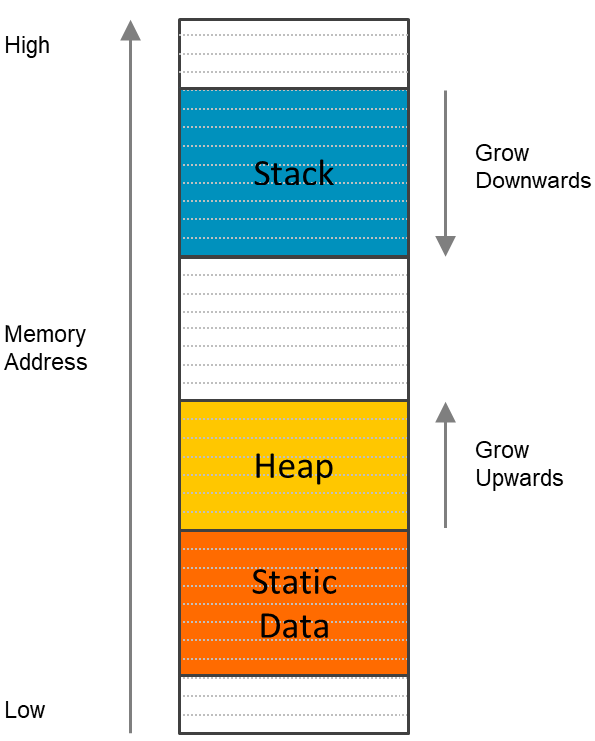
\includegraphics[width=\linewidth]{images/ram1.png}
\end{minipage}
\begin{minipage}{.49\columnwidth}
    \centering
    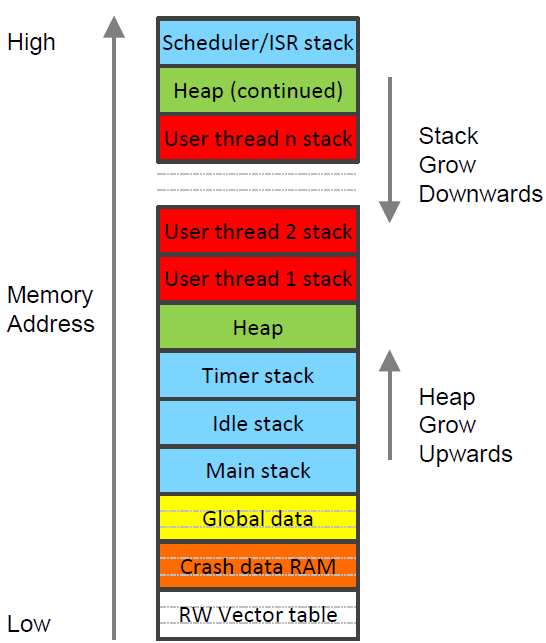
\includegraphics[width=\linewidth,height=\linewidth,keepaspectratio=false]{images/ram2.png} % set height to \linewidth
\end{minipage}\\
Typically, the data can be divided into three
sections: static data, stack, and heap:
\begin{itemize}
    \item Static data: contains global variables and static variables
    \item Stack: contains the temporary data for local variables, parameter passing in function calls, registers saving during exceptions, etc.
    \item Heap: contains the pieces of memory spaces that are dynamically reserved by calloc() malloc() or new calls.
\end{itemize}
\includegraphics*[width=\columnwidth]{images/datastorage_example.png}
Can the information change?
\begin{itemize}
    \item No: put it in read-only, nonvolatile memory for saving RAM
    \item Yes: put it in read/write memory
\end{itemize}
How long does the data need to exist?
\begin{itemize}
    \item Program scope: statically allocated
    \item Function/method scope: automatically allocated on the stack
    \item From explicit allocation to explicit deallocation: on the heap
    \item Always define the most restrictive scope
    \item Use dynamic allocation on the heap with care
\end{itemize}
\underline{Class qualifiers and data type:}\\
\includegraphics*[width=\columnwidth]{images/data_types.png}
\begin{itemize}
    \item \texttt{const}: the value of the variable cannot be changed after initialization.
          Never written by program, can be put in ROM to save RAM.
    \item \texttt{volatile}: the value of the variable can be changed by external events.
          Can be changed outside of normal program flow: ISR, hardware register
          Compiler must be careful with optimizations.
    \item \texttt{static}: the variable is shared between all instances of the class.
          Declared within function or method, retains value between function/method invocations
          Declared within classes: the field is instantiated once for all class instances and the value
          is retained for the program lifetime.
\end{itemize}
\underline{Memory hierarchy:}\\
\includegraphics*[width=\columnwidth]{images/memory_hierarchy.png}
\begin{itemize}[itemsep=0pt, topsep=0pt, partopsep=0pt]
    \item Register: usually one CPU cycle to access
    \item Cache: Static RAM
    \item Main Memory: Dynamic RAM, Volatile data
    \item Secondary Memory: Flash/Hard disk
    \item Tertiary Memory: Tape libraries
\end{itemize}
    \subsection*{Bootloader}
A Bootloader is a program that runs when a device is powered on or reset. It is responsible for
loading the operating system kernel to memory and starting its execution. It is usually stored in
the non-volatile memory of the device. Primary purpose: allow a software/firmware to be
updated without the use of specialized hardware (No JTAG programmer).

\end{multicols*}
\end{document}